\begin{figure}
  \centering
  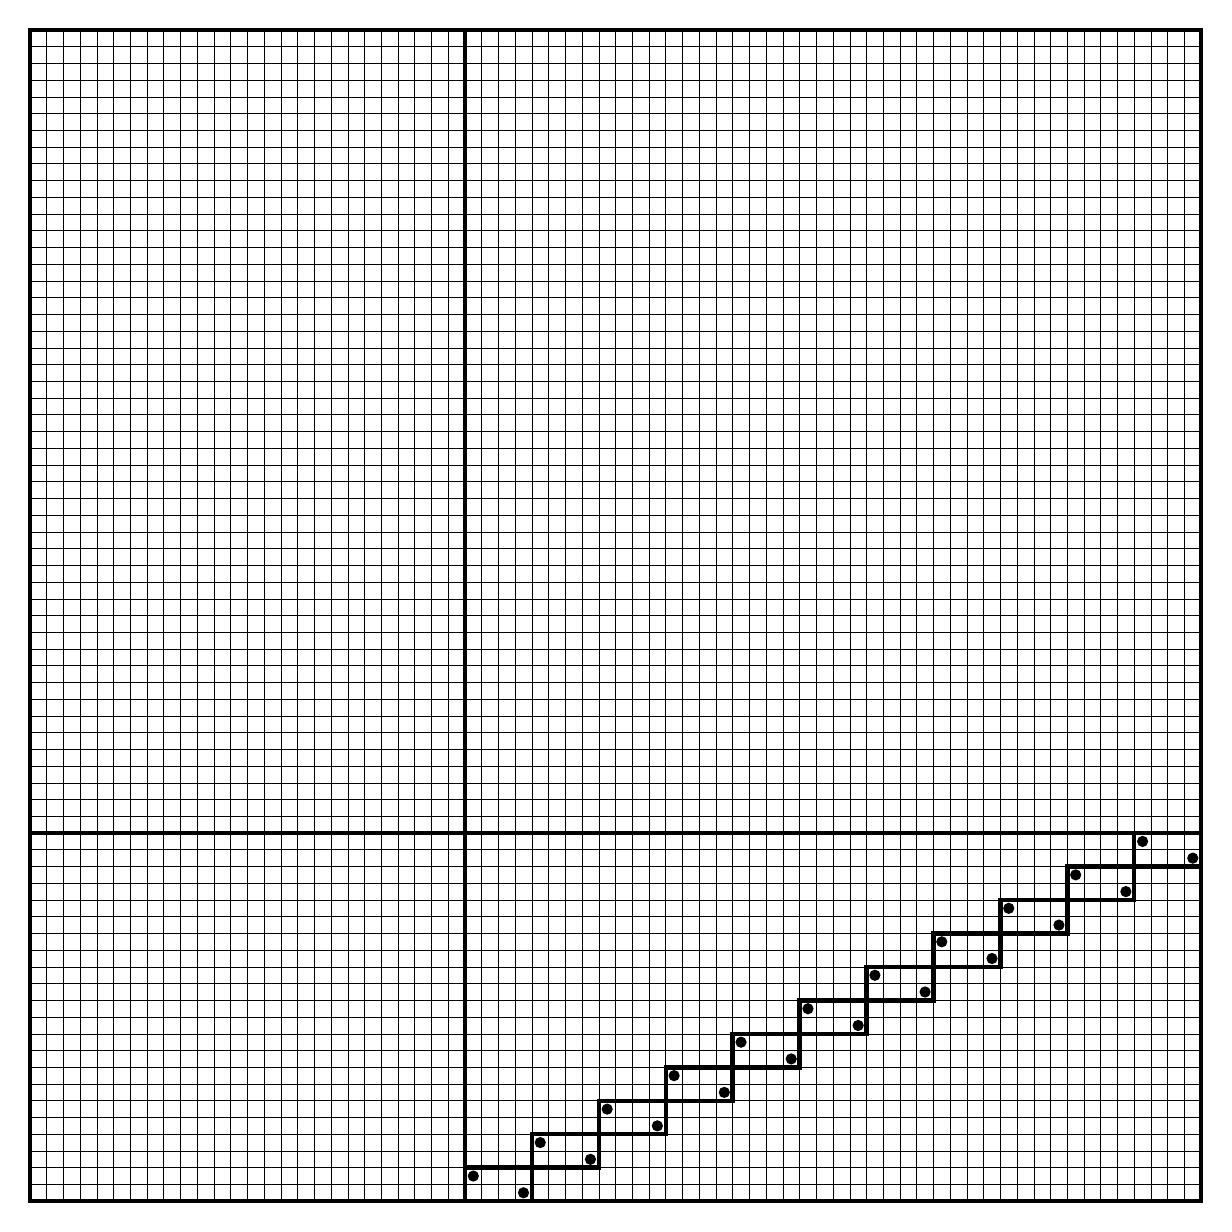
\begin{tikzpicture}
  [
    scale=.425,
    box/.style={
      shade,
      blur shadow={shadow blur steps=5,shadow blur extra rounding=1.3pt},
      top color=black!5,
      bottom color=black!50
    },
    gadget/.style={
      box,
      rounded corners
    },
    r/.style={
      box,
      draw,
      ultra thick,
    }
  ]

  \draw [very thin,step=0.5cm] (0,0) grid (35,35);
  \draw [ultra thick] (0,0) rectangle (35,35);

  \draw [ultra thick] (0,11) -- (35,11);
  \draw [ultra thick] (13,0) -- (13,35);

  \foreach \e in {1,2,...,11} {
      \draw [ultra thick] (11 + \e*2, -1 + \e) rectangle (13 + \e*2, \e);
      \draw [fill=black] (11.25 + \e*2, -.25 + \e) circle (0.15);
      \draw [fill=black] (12.75 + \e*2, -.75 + \e) circle (0.15);
  }

  \end{tikzpicture}
\end{figure}
